\begin{wrapfigure}{r}{0.5\textwidth}
    %\begin{figure}[hbt]
    \vspace{-20pt}
    \centering
    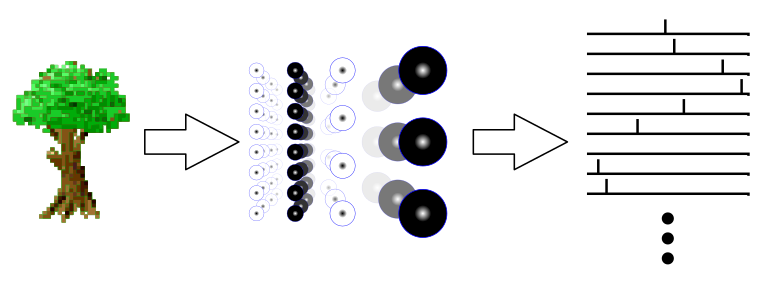
\includegraphics[width=0.5\textwidth]{model-schematic}
    \caption{Schematic of the foveal pit model}
    \label{pic-fov-pit-model}
    %\end{figure}
\end{wrapfigure}

A functional model is one that treats a system as a black box
and tries to ``map'' observed inputs to their respective outputs 
by means of a set of mathematical expressions. The model created
by \citeauthor{basab-model} in \cite{basab-thesis, basab-model},
consists of several instances of four ganglion cells (midget and 
parasol, with ON and OFF centres) which transform the pixels in 
the received image into rank-ordered spike trains (Figure 
\ref{pic-fov-pit-model}). This model is based on previous work 
by \citeauthor{van-rullen-rate-coding} in
\cite{van-rullen-rate-coding}.


\subsubsection{Neural codes} There are many ways of encoding 
information using spikes. The most common one is rate-based, in 
which the average count of spikes fired by a neuron encodes a value. 
A different approach is to take the exact timing of spikes when 
they were generated as a means to transmit information. The latter 
has great encoding capabilities since there are many times in which 
a spike can occur. Rate-based codes tend to have limited 
representational power because the same spike count can happen due
to different inputs.

A simpler way of encoding spikes is to not really pretend to know 
exactly when they where actually emitted, but to just take into 
account the order in which they happened; this is referred as a 
rank-ordered encoding. This code has the advantage of being able 
to transmit more information than rate-based ones 
\cite{basab-thesis,thorpe-spike-rapid-processing, thorpe-rate-coding-theory}, 
yet maintain a simple way of interpretation. Furthermore, rank-ordered
encoding has shown to provide enough information for reconstruction
in about the highest 20 to 30\% spikes.


\subsubsection{Mathematical model} As discussed in section \ref{sec-retina},
the Foveal pit region of the retina is the highest resolution 
zone in the retina. This is taken into account by simulating one 
midget cell per pixel and one parasol cell about every 7 pixels.

Each ganglion cell is characterized by a Difference of Gaussian 
(DoG), described in equation \ref{eq-dog}. 

\begin{equation}
\label{eq-dog}
DoG_w(x,y) = \pm\frac{1}{2\pi\sigma_{w,c}^2}e^{\frac{-(x^2 + y^2)}{2\sigma_{w,c}^2}}
             \mp\frac{1}{2\pi\sigma_{w,s}^2}e^{\frac{-(x^2 + y^2)}{2\sigma_{w,s}^2}}
\end{equation}

where $\sigma_{w,c}$ and $\sigma_{w,s}$ are the standard deviation 
for the centre and surround components of the DoG at scale $w$ 
(cell type). The signs will be ($-$,$+$) if the 
ganglion cell is OFF-centre; ($+$,$-$) if it is ON-centre. The simulation 
of a cell is carried by a discrete convolution 
(Eq. \ref{eq-convolution}) of a DoG over the input image.

\begin{equation}
\label{eq-convolution}
C(x,y,w) = \sum_i \sum_j \left( I(i+x, j+y) \cdot DoG_w(i,j)\right)
\end{equation}

This will provide a set of coefficients $C$ for every scale $w$. 
The authors in \cite{van-rullen-rate-coding} refer to this as a 
wavelet-like transformation. The value of the coefficient will mean 
how soon does the neuron fire. If all $c_{i,w}$ are sorted according to their 
value, we shall posses a rank-ordered spikes set.\\

Cells are parametrized according to table \ref{tb-ganglion}. After
applying discrete convolutions to a test image Fig. \ref{pic-lena}, 
the results can be seen in Figs. \ref{pic-lena-M-OFF}, \ref{pic-lena-M-ON}
\ref{pic-lena-P-OFF} and \ref{pic-lena-P-ON}.

\begin{table}[hb]
    \caption{Simulation parameters for ganglion cells}
    \centering
\begin{TAB}(r,1em,1.5em){|c|c|c|c|c|}{|c|c|c|c|c|} 
    Cell type & Matrix size &  Centre std. dev. ($\sigma_c$) & 
    Surround std. dev. ($\sigma_s$)  & Sampling resolution  \\
    Midget OFF-centre  & $3 \times 3$ & $0.8$ & $6.7 \times \sigma_c$ &  col: 1, row: 1\\
    Midget ON-centre   & $11 \times 11$ & $1.04$ & $6.7 \times \sigma_c$ &  col: 1, row: 1\\
    Parasol OFF-centre & $61 \times 61$ & $8$ & $4.8 \times \sigma_c$ & col: 5, row: 3 \\
    Parasol ON-centre  & $243 \times 243$ & $10.4$ & $4.8 \times \sigma_c$ & col: 5, row: 3 \\
\end{TAB} 
\label{tb-ganglion}
\end{table}


\begin{figure}[hbt]
    \centering
    \begin{subfigure}[t]{0.15\textwidth}
        \centering
        \captionsetup{justification=centering,margin=0.1cm}
        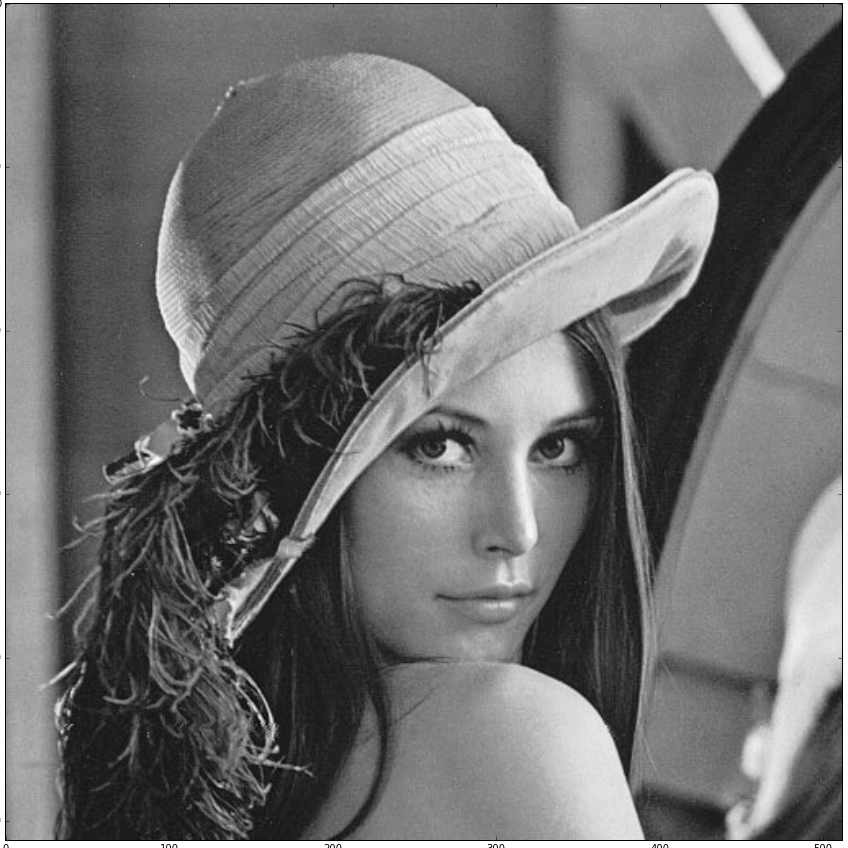
\includegraphics[width=\textwidth]{./Lena-gray}
        \caption{\\Original image}
        \label{pic-lena}
    \end{subfigure}
    \begin{subfigure}[t]{0.15\textwidth}
        \centering
        \captionsetup{justification=centering,margin=0.1cm}
        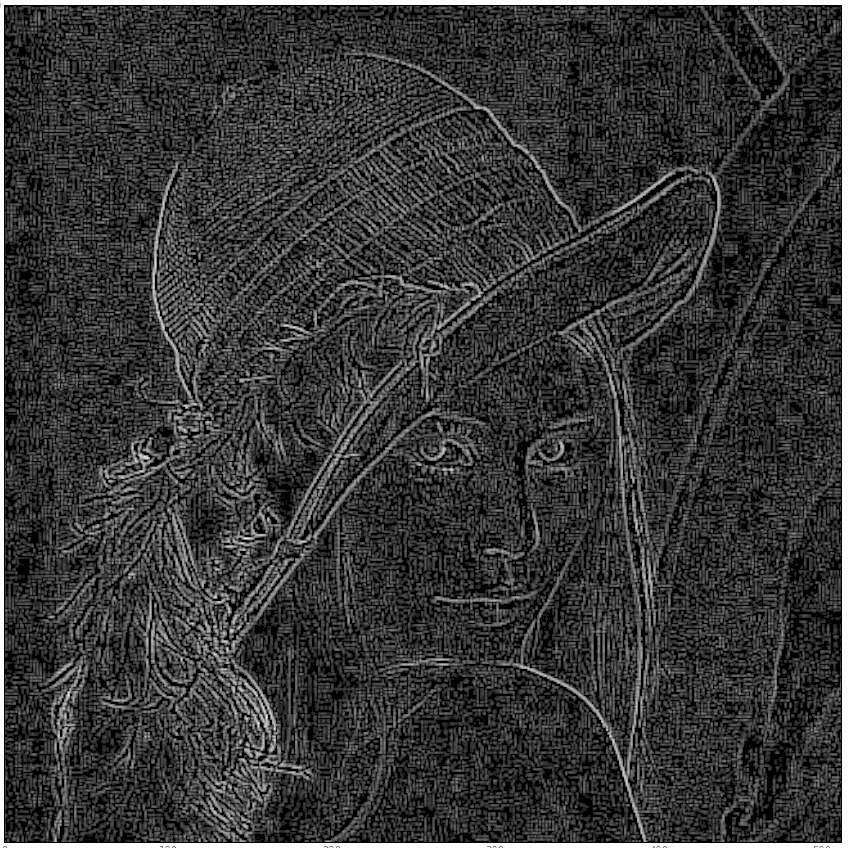
\includegraphics[width=\textwidth]{./Lena-midget_off}
        \caption{\\Midget OFF-centre}
        \label{pic-lena-M-OFF}
    \end{subfigure}
    \begin{subfigure}[t]{0.15\textwidth}
        \centering
        \captionsetup{justification=centering,margin=0.1cm}
        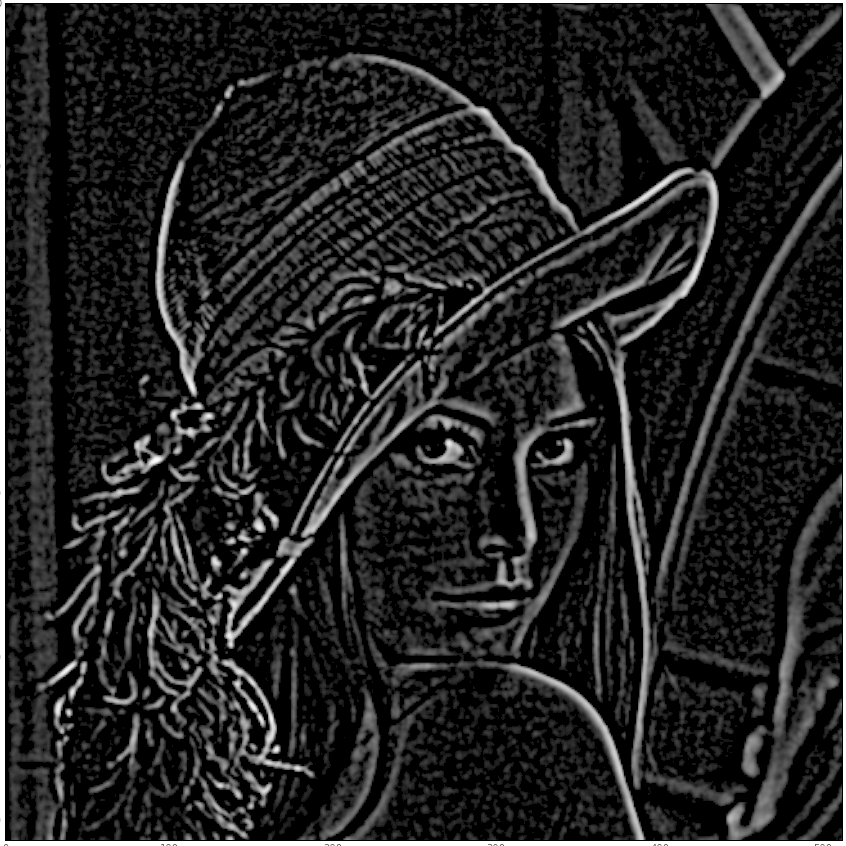
\includegraphics[width=\textwidth]{./Lena-midget_on}
        \caption{\\Midget ON-centre}
        \label{pic-lena-M-ON}
    \end{subfigure}
    \begin{subfigure}[t]{0.15\textwidth}
        \centering
        \captionsetup{justification=centering,margin=0.1cm}
        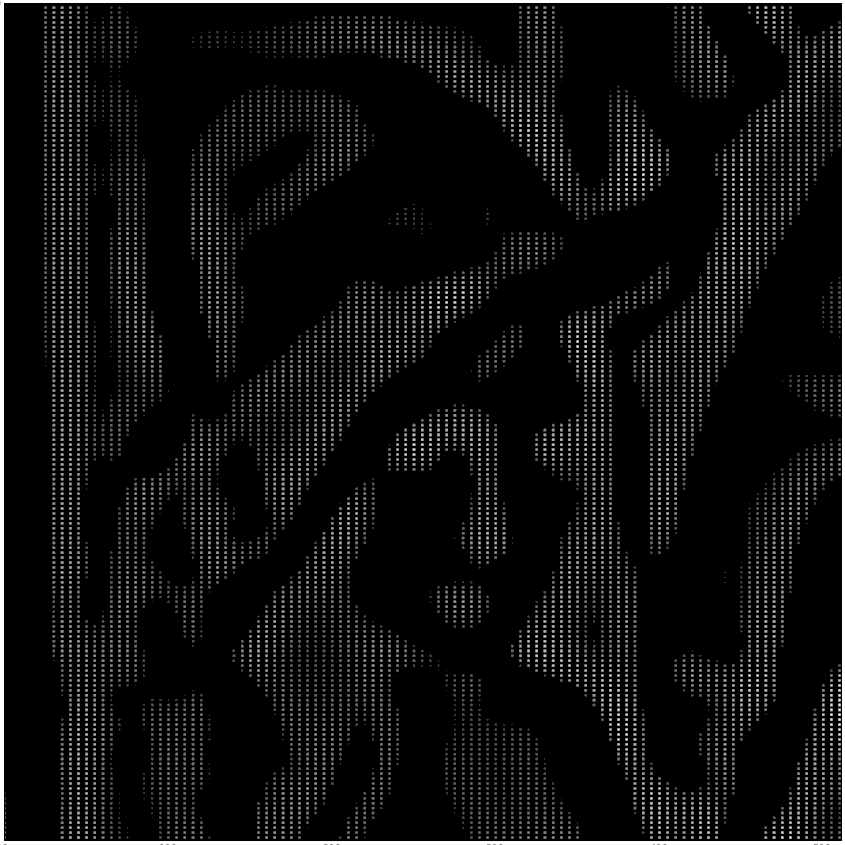
\includegraphics[width=\textwidth]{./Lena-parasol_off}
        \caption{\\Parasol OFF-centre}
        \label{pic-lena-P-OFF}
    \end{subfigure}
    \begin{subfigure}[t]{0.15\textwidth}
        \centering
        \captionsetup{justification=centering,margin=0.1cm}
        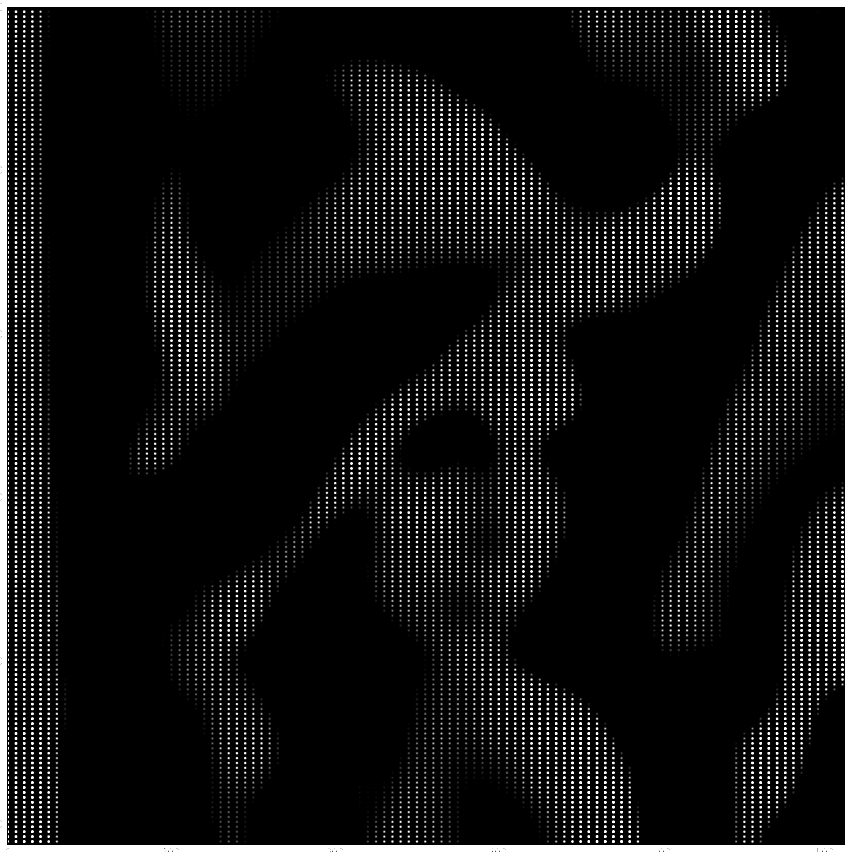
\includegraphics[width=\textwidth]{./Lena-parasol_on}
        \caption{\\Parasol ON-centre}
        \label{pic-lena-P-ON}
    \end{subfigure}
    \caption{Results of simulating ganglion cells (convoluted images, enhanced for better contrast)}
\end{figure}
